\documentclass[letterpaper,12pt,oneside]{article}\usepackage[]{graphicx}\usepackage[]{color}
%% maxwidth is the original width if it is less than linewidth
%% otherwise use linewidth (to make sure the graphics do not exceed the margin)
\makeatletter
\def\maxwidth{ %
  \ifdim\Gin@nat@width>\linewidth
    \linewidth
  \else
    \Gin@nat@width
  \fi
}
\makeatother

\definecolor{fgcolor}{rgb}{0.345, 0.345, 0.345}
\newcommand{\hlnum}[1]{\textcolor[rgb]{0.686,0.059,0.569}{#1}}%
\newcommand{\hlstr}[1]{\textcolor[rgb]{0.192,0.494,0.8}{#1}}%
\newcommand{\hlcom}[1]{\textcolor[rgb]{0.678,0.584,0.686}{\textit{#1}}}%
\newcommand{\hlopt}[1]{\textcolor[rgb]{0,0,0}{#1}}%
\newcommand{\hlstd}[1]{\textcolor[rgb]{0.345,0.345,0.345}{#1}}%
\newcommand{\hlkwa}[1]{\textcolor[rgb]{0.161,0.373,0.58}{\textbf{#1}}}%
\newcommand{\hlkwb}[1]{\textcolor[rgb]{0.69,0.353,0.396}{#1}}%
\newcommand{\hlkwc}[1]{\textcolor[rgb]{0.333,0.667,0.333}{#1}}%
\newcommand{\hlkwd}[1]{\textcolor[rgb]{0.737,0.353,0.396}{\textbf{#1}}}%

\usepackage{framed}
\makeatletter
\newenvironment{kframe}{%
 \def\at@end@of@kframe{}%
 \ifinner\ifhmode%
  \def\at@end@of@kframe{\end{minipage}}%
  \begin{minipage}{\columnwidth}%
 \fi\fi%
 \def\FrameCommand##1{\hskip\@totalleftmargin \hskip-\fboxsep
 \colorbox{shadecolor}{##1}\hskip-\fboxsep
     % There is no \\@totalrightmargin, so:
     \hskip-\linewidth \hskip-\@totalleftmargin \hskip\columnwidth}%
 \MakeFramed {\advance\hsize-\width
   \@totalleftmargin\z@ \linewidth\hsize
   \@setminipage}}%
 {\par\unskip\endMakeFramed%
 \at@end@of@kframe}
\makeatother

\definecolor{shadecolor}{rgb}{.97, .97, .97}
\definecolor{messagecolor}{rgb}{0, 0, 0}
\definecolor{warningcolor}{rgb}{1, 0, 1}
\definecolor{errorcolor}{rgb}{1, 0, 0}
\newenvironment{knitrout}{}{} % an empty environment to be redefined in TeX

\usepackage{alltt}
\usepackage[paperwidth=8.5in,paperheight=11in,top=1in,bottom=1in,left=1in,right=1in]{geometry}
\usepackage{setspace}
\usepackage[colorlinks=true,allcolors=Blue]{hyperref}
\usepackage[usenames,dvipsnames]{xcolor}
\usepackage{indentfirst}
\usepackage{titlesec}
\usepackage{multirow}
\usepackage{booktabs}
\usepackage{graphicx}
\usepackage{verbatim}
\usepackage{rotating}
\usepackage{tabularx}
\usepackage{outlines}
\usepackage{lineno}
\usepackage{array}
\usepackage{times}
\usepackage{cleveref}
\usepackage{acronym}
\usepackage[position=t]{subfig}
\usepackage{paralist}
\usepackage[noae]{Sweave}
\usepackage{natbib}
\usepackage{array}
\usepackage{pdflscape}
\usepackage{bm}
% \usepackage{showlabels}
\bibpunct{(}{)}{,}{a}{}{,}

% page margins and section title formatting
\linespread{1.5}
\setlength{\footskip}{0.5in}
\titleformat*{\section}{\Large\bf\em}
\titleformat*{\subsection}{\singlespace\large\bf}
\titleformat*{\subsubsection}{\singlespace\normalsize\bf\em}
\titlespacing{\section}{0in}{0in}{0in}
\titlespacing{\subsection}{0in}{0in}{0in}
\titlespacing{\subsubsection}{0in}{0in}{0in}

% cleveref options
\crefname{table}{Table}{Tables}
\crefname{figure}{Fig.}{Figs.}
\renewcommand{\figurename}{Fig.}

% aliased citations
% \defcitealias{FLDEP12}{FLDEP 2012}

%acronyms
\acrodef{sfe}[SFE]{San Francisco Estuary}
\acrodef{wrtds}[WRTDS]{Weighted Regressions on Time, Discharge, and Season}

%for supplemental figures/tables
\newcommand{\beginsupplement}{%
        \setcounter{table}{0}
        \renewcommand{\thetable}{S\arabic{table}}%
        \setcounter{figure}{0}
        \renewcommand{\thefigure}{S\arabic{figure}}%
     }

%knitr options


% get the version based on commit date


% get online bib file


\IfFileExists{upquote.sty}{\usepackage{upquote}}{}
\begin{document}

\raggedbottom
\linenumbers
\raggedright
\urlstyle{same}
\setlength{\parindent}{0.5in}
\renewcommand\refname{References \vspace{12pt}}

\begin{singlespace}
\title{{\bf {\Large Four decades of water quality changes in the upper San Francisco Estuary}}}
\author{
  {\bf {\normalsize Marcus W. Beck$^1$, David Senn$^2$, Phil Bresnahan$^2$, Emily Novick$^2$, James D. Hagy III$^1$,}}
  \\{\bf {\normalsize Thomas Jabusch$^2$}}
  \\\\{\textit {\normalsize $^1$USEPA National Health and Environmental Effects Research Laboratory}}
  \\{\textit {\normalsize Gulf Ecology Division, 1 Sabine Island Drive, Gulf Breeze, FL 32561}}
	\\{\textit {\normalsize Phone: 850-934-2480, Fax: 850-934-2401}}
	\\{\textit {\normalsize Emails: \href{mailto:beck.marcus@epa.gov}{beck.marcus@epa.gov}, \href{mailto:hagy.jim@epa.gov}{hagy.jim@epa.gov}}}
  \\\\{\textit {\normalsize $^2$San Francisco Estuary Institute}}
	\\{\textit {\normalsize 4911 Central Avenue, Richmond, CA 94804}}
	\\{\textit {\normalsize Phone: 510-746-7334, Fax: 510-746-7300}}
	\\{\textit {\normalsize Emails: \href{mailto:davids@sfei.org}{davids@sfei.org}, \href{mailto:philb@sfei.org}{philb@sfei.org}, \href{mailto:emilyn@sfei.org}{emilyn@sfei.org}, \href{mailto:thomasj@sfei.org}{thomasj@sfei.org}}}
  \vspace{1in} 
  \\ Version Date:   Wed May 25 08:44:44 2016 -0500
	}
\date{}
\maketitle
\end{singlespace}
\clearpage

\begin{abstract}
\noindent Recent methods for trend analysis have been developed that leverage the descriptive potential of long-term time series.  Combined with these methods, multi-decadal datasets of water quality in coastal systems can provide valuable opportunities to gain insight into ecosystem properties and drivers of change.  This study describes the application of an estuarine adaptation of the \ac{wrtds} approach to describe water quality trends in the upper region of the \ac{sfe}, a primary source of nutrients into the system.  This statistical technique is data-driven where the parameterization of the functional model changes smoothly over time following dynamic patterns of season and flow.  By doing so, changes over time that have not been previously quantified can be described, including variation in flow-normalized concentrations, frequency occurrence of extreme events, and response to historical changes in the watershed, all of which are important needs for understanding trends in the \ac{sfe}.  The goal of the analysis is to apply the WRTDS model at multiple stations in the Delta and Suisun Bay regions of \ac{sfe} to provide novel descriptions of water quality changes over time and relationships between key species of dissolved inorganic nitrogen (ammonium, nitrate/nitrite, total).  This variation is considered in the context of varying contributions of input flows from the Sacramento and San Joaquin rivers, as well as tidal exchange with the central \ac{sfe}.  The results are described in the context of conceptual relationships between water quality and drivers of change to generate hypotheses of mechanistic relationships using selected examples from the trend descriptions. Overall, this analysis provides an ecological and management-based understanding of historical trends in the \ac{sfe} as a means to interpret potential impacts of recent changes and expected trends in this dynamic system.  An argument is also made for more comprehensive evaluations of long-term monitoring datasets to understand relationships between response endpoints and causal mechanisms in coastal waters.
\end{abstract}
\acresetall

\section{Introduction}

\begin{itemize}
\item Paragraph 1 - how and why are trends interpreted - raw data, surrogates, various methods, what have been implications of using different approaches
\item Paragraph 2 - WRTDS for estuaries, application to Tampa Bay as test set, further validation in Patuxent
\item Paragraph 3 - SF estuary, unique and prominent location, full story is not known (historical context and recent changes), no one has empirically described the data, how is this related to the delta (a vigorous biogeochemical reactor)
\item Paragraph 4 - Study goal and objectives
\begin{itemize}
\item Provide a description of trends - annual, seasonal, spatial, response to flow, change by analytes
\item Detailed description of selected sites in the context of conceptual relationships - 1) nonlinear or extreme quantile changes site TBD, 2) P8 and WWTP improvements, 3) Suisun DIN, SiO2, Chla, and clams
\item What this means for understanding other systems
\end{itemize}
\end{itemize}

\section{Methods}

\begin{itemize}
\item Study location and data - describe conceptual relationships
\item WRTDS method - estuarine adaptation, how was it applied to \ac{sfe}
\end{itemize}

\section{Results}

\section{Discussuion}

What additional information is needed?

method leads to hypothesis generation or mechanistic explanations of change, verification of conceptual links

\begin{figure}
\centering
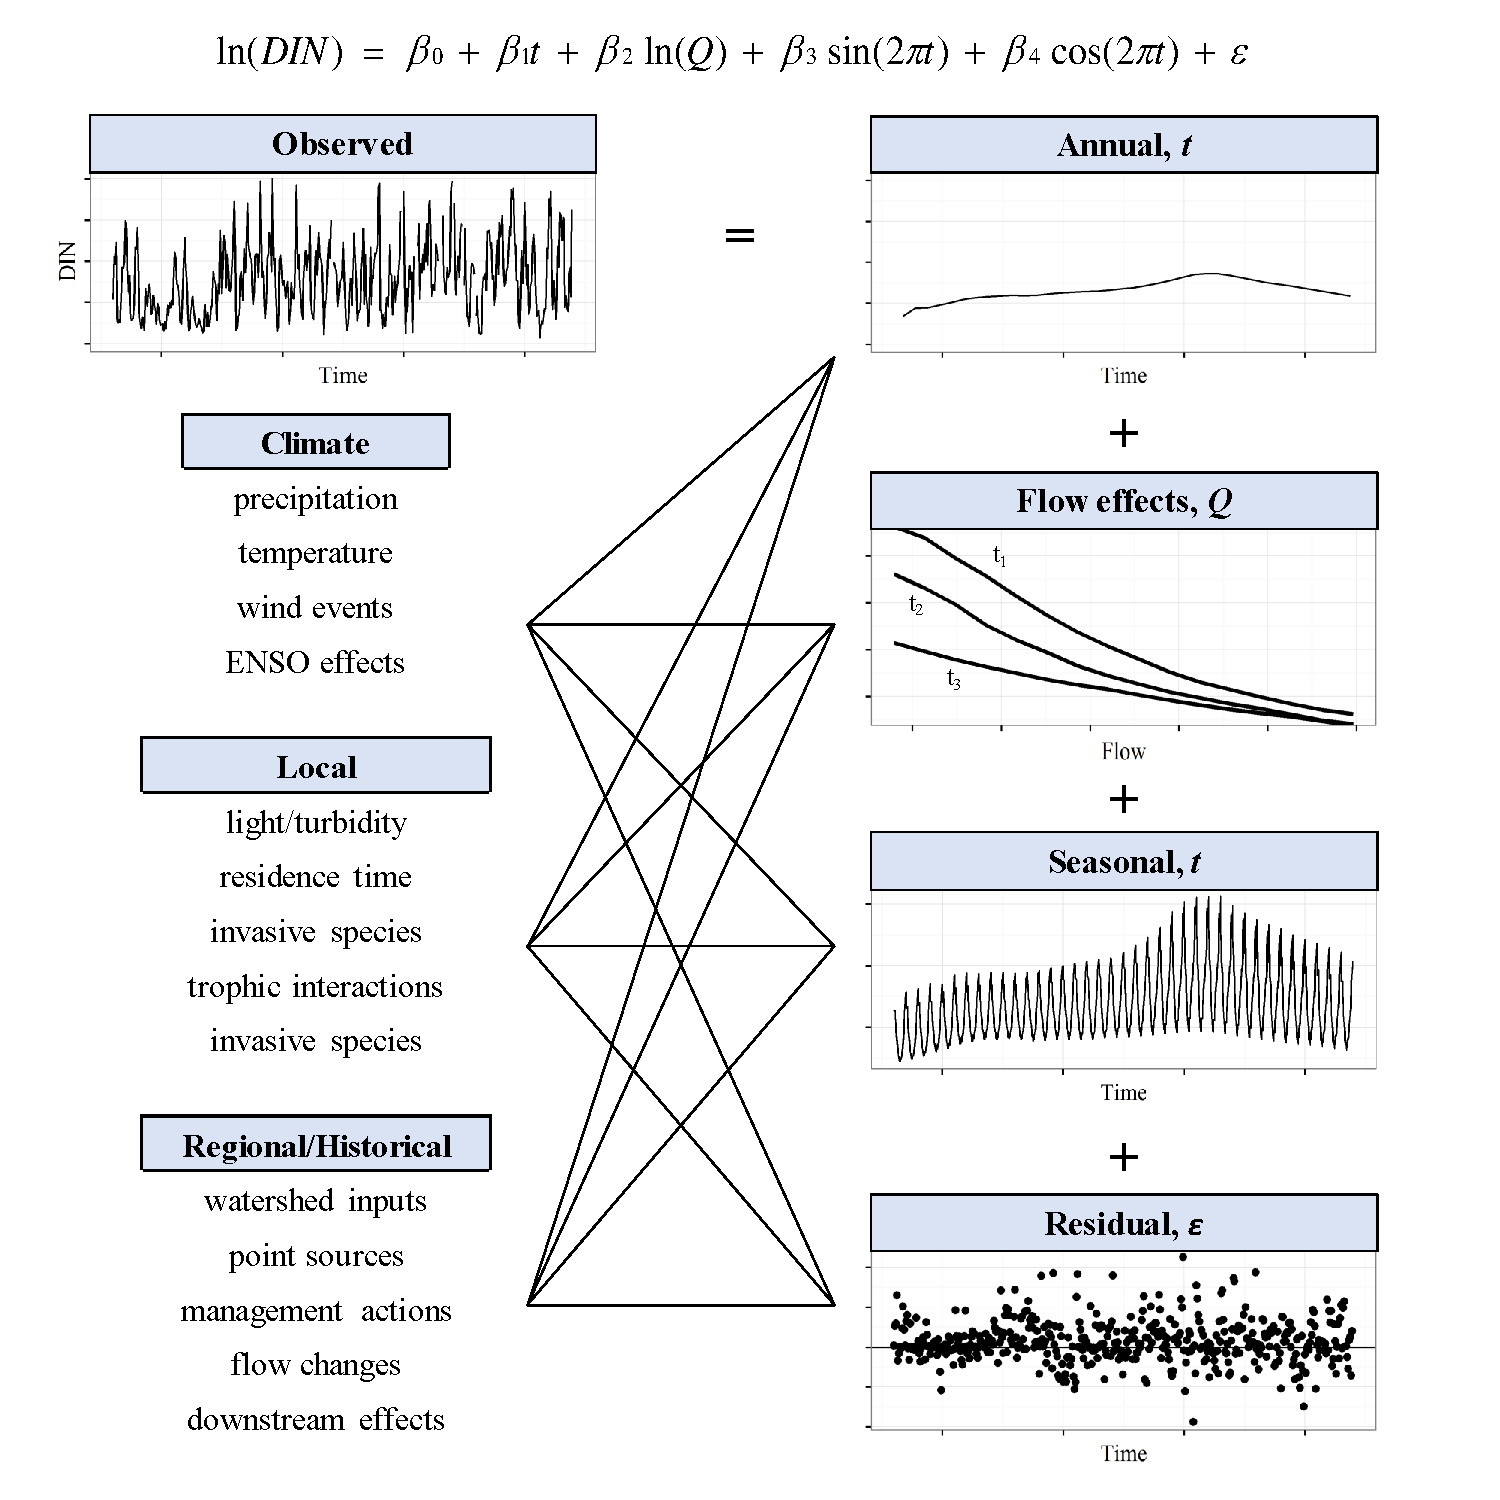
\includegraphics[width=1\textwidth,page=1]{figs/schematic.pdf}
\caption{schematic}
\label{fig:schematic}
\end{figure}

\end{document}
